\documentclass[12pt]{article}
\usepackage{tikz}
\usetikzlibrary{bayesnet}
\usepackage{amsmath}
\begin{document}
\section*{Divisive Normalization Notes}
We consider the problem of demixing stimuli that are mixed due to neurons having large receptive fields or wide tuning curves.
\subsection{Generative model}
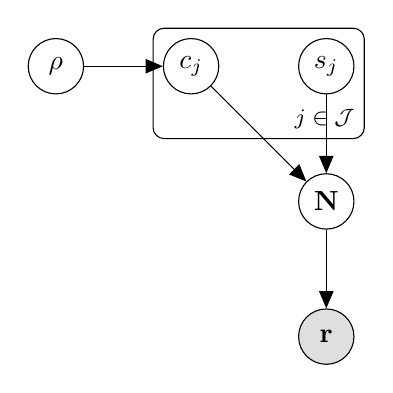
\begin{tikzpicture}
\node[obs]                               (r) {$\mathbf{r}$};
  \node[latent, above=of r]        (N) {$\mathbf{N}$};
  \node[latent, above=of N] (s) {$s_j$};
   \node[latent, left=of s]  (c) {$c_j$};
  \node[latent, left=of c]  (rho) {$\rho$};
   \edge {c,s} {N};
  \edge {N} {r}; 
  \edge {rho} {c}; 
  \plate {} {(c) (s)} {$j \in \mathcal{J}$};
 \end{tikzpicture}
 \\
$s_j$ is the $j^\text{th}$ stimulus, $\mathbf{s} \sim \text{Unif} (0, \pi)$\\
$c_j$ is the contrast of the $j^\text{th}$ stimulus, $\mathbf{c} \sim \text{Dir} (\rho)$\\
~\\
$f_i(s)$ is the tuning curve of the $i^\text{th}$ neuron in response to a single stimulus $s$\\
Tuning curve assumptions:
\begin{itemize}
\item Tuning curves cover the space so $\sum_i f_i(s)$ is independent of $s$
\item The tuning curves are Gaussian: $f_i(s_j) \sim \mathcal{N} (s_i^{\text{pref}}, \sigma_{\text{tc}}^2)$
\end{itemize}
$N_{ij}$ is the spike count of the $i^\text{th}$ neuron elicited by the $j^\text{th}$ stimulus\\
$N_{ij}|s_j  \sim \text{Poisson}(c_j f_i(s_j))$\\
$r_i$ is the total spike count of the $i^\text{th}$ neuron in response to all stimuli\\
$r_i = \sum_j N_{ij}$\\

\subsection{Inference}
\begin{equation}
\begin{aligned}
P(\mathbf{c, s|r}) & = \sum_\mathbf{N} P(\mathbf{N, c, s|r}) \\
P(\mathbf{N, c, s|r}) 
& =  P(\mathbf{r|N}) P(\mathbf{N|c, s}) P(\mathbf{c}) P(\mathbf{s})\\
&\propto \prod_i \left[\delta \Big( r_i - \sum_j N_{ij} \Big) \bigg( \prod_j\frac{(f_i(s_j)c_j)^{N_{ij}}}{N_{ij}!} \bigg) \right] \prod_j \frac{1}{\mathbf{\beta}(\rho)} c_j^{\rho_j - 1} 
\end{aligned}
\end{equation}
For the variational inference, we need\\
 \begin{equation}
\begin{aligned}
\log P(\mathbf{N, c, s| r}) &= \sum_i \Big[ \log\delta \Big( r_i - \sum_j N_{ij} \Big) + \sum_j \big[-\log N_{ij}! + N_{ij} \log(f_i(s_j)c_j)\big] \Big]\\
& \phantom{{}=1} + \sum_j (\rho_j - 1)\log c_j
\end{aligned}
\end{equation}
\subsection{Variational approximation}
Then we approximate this using a factorized distribution:
\begin{equation}
Q(\mathbf{N, c, s|r}) = Q(\mathbf{N|r}) Q(\mathbf{c|r}) Q(\mathbf{s|r})
\end{equation}
\begin{equation}
\begin{aligned}
\log Q(\mathbf{N}|\mathbf{r}) &= \sum_i \log Q(\mathbf{N}_i|\mathbf{r}_i)\\
\log Q(\mathbf{N}_i|\mathbf{r}_i) &= \langle \log P(\mathbf{N_i, c, s|r_i}) \rangle_{Q(\mathbf{c|r})Q(\mathbf{s|r})}\\
&= \log(\delta \Big( r_i - \sum_j N_{ij} \Big) + \sum_j N_{ij}\big( \langle \log c_j \rangle + \langle \log f_i(s_j) \rangle \big) - \sum_j \log N_{ij}!\\
\log Q(\mathbf{c|r}) &= \langle \log P(\mathbf{N, c, s|r}) \rangle_{Q(\mathbf{N|r})Q(\mathbf{s|r})}\\
&= \sum_j [\log (c_j \rho_j - 1) + \sum_i \langle N_{ij} \rangle_{Q(\mathbf{N|r})}]\\
\log Q(\mathbf{s|r}) &= \langle \log P(\mathbf{N, c, s|r}) \rangle_{Q(\mathbf{N|r})Q(\mathbf{c|r})}\\
&= \sum_{ij} [\langle N_{ij} \rangle_{Q(\mathbf{N|r})} \log(f_i(s_j)) - f_i(s_j) \langle c_j \rangle_{Q(\mathbf{c|r})}]\\ 
&= \sum_{ij} \langle N_{ij} \rangle_{Q(\mathbf{N|r})} \log(f_i(s_j))
\end{aligned}
\end{equation}
So we now know
\begin{equation}
\begin{aligned}
Q(\mathbf{c|r}) &\sim \text{Dir}(\boldsymbol{\alpha})\\
\alpha_j &= \rho_j - 1 + \sum_i \langle N_{ij} \rangle_{Q(\mathbf{N|r})}\\
\end{aligned}
\end{equation}
and 
\begin{equation}
\begin{aligned}
Q(s_j|r) &\propto \frac{1}{2 \sigma_{\text{tc}}^2} \sum_{i=1}^I \langle N_{ij} \rangle_{Q(\mathbf{N|r})} (s_j - s_i^{\text{pref}})^2\\
&\sim \mathcal{N} (\mu_j, \tau_j)\\ 
\tau_j &= \sum_{i=1}^I \frac{\langle N_{ij} \rangle_{Q(\mathbf{N|r})}}{2 \sigma_{\text{tc}}^2}\\
\mu_j &= \frac{1}{\tau_j} \sum_{i=1}^I s_i^{\text{pref}} \frac{\langle N_{ij} \rangle_{Q(\mathbf{N|r})}}{2 \sigma_{\text{tc}}^2}\\
\end{aligned}
\end{equation}
\begin{equation}
\begin{aligned}
Q(N_{ij}|r) &\sim \text{Mult}(r_i, p_{ij})\\
p_{ij} &= \frac{e^{\langle \log c_j \rangle + \langle \log f_i(s_j) \rangle}}{\sum_{j=1}^J e^{\langle \log c_j \rangle + \langle \log f_i(s_j) \rangle}}\\
\end{aligned}
\end{equation}
From this we can compute:
\begin{equation}
\langle \log c_j \rangle_{Q(c_j)}= \Psi(\alpha_j) - \Psi(\sum_{j=1}^J \alpha_j)
\end{equation}
and
\begin{equation}
\begin{aligned}
\langle \log f_i(s_j) \rangle_{Q(s_j)} &= \frac{-\langle (s_j - s_i^{\text{pref}})^2 \rangle_{Q(s_j)}}{2 \sigma_{\text{tc}}^2}\\
&=  \frac{-[(s_i^{\text{pref}} - \mu_j)^2 + \tau_j^{^{-1}}]}{2 \sigma_{\text{tc}}^2}
\end{aligned}
\end{equation}
Therefore: 
\begin{equation}
p_{ij} = \frac{e^{\Psi(\alpha_j) - \Psi(\sum_{j=1}^J \alpha_j) - \frac{(s_i^{\text{pref}} - \mu_j)^2 + \tau_j^{-1}}{2 \sigma_{\text{tc}}^2}}}{\sum_{j=1}^J e^{\Psi(\alpha_j) - \Psi(\sum_{j=1}^J \alpha_j) - \frac{(s_i^{\text{pref}} - \mu_j)^2 + \tau_j^{-1}}{2 \sigma_{\text{tc}}^2}}}
\end{equation}
\begin{equation}
\alpha_j = \rho_j - 1 + \sum_i r_i p_{ij}
\end{equation}
\begin{equation}
\tau_j = \sum_{i=1}^I \frac{r_i p_{ij}}{2 \sigma_{\text{tc}}^2}
\end{equation}
\begin{equation}
\mu_j = \frac{1}{\tau_j} \sum_{i=1}^I s_i^{\text{pref}} \frac{r_i p_{ij}}{2 \sigma_{\text{tc}}^2}
\end{equation}
We actually want the natural parameters so 
\begin{equation}
\eta_j = \mu_j \tau_j = \sum_{i=1}^I s_i^{\text{pref}} \frac{r_i p_{ij}}{2 \sigma_{\text{tc}}^2}
\end{equation}
Also we don't want complex division in the neural computations so:
\begin{equation}
\begin{aligned}
F_i(\mu_j, \alpha_j, \tau_j) &= e^{\Psi(\alpha_j) - \Psi(\sum_{j=1}^J \alpha_j) - \frac{(s_i^{\text{pref}} - \frac{\eta_j}{\tau_j})^2 + \tau_j^{-1}}{2 \sigma_{\text{tc}}^2}}\\
p_{ij} &= F_i(\mu_j, \alpha_j, \tau_j) \pi_i\\
\pi_i &= \frac{1}{\sum_{j=1}^J F_i(\mu_j, \alpha_j, \tau_j)}
\end{aligned}
\end{equation}

And now we have update equations: 
\begin{equation}
\begin{aligned}
\frac{d \eta_j}{dt} &= - \eta_j + \frac{1}{2 \sigma_{\text{tc}}^2} \sum_{i=1}^I s_i^{\text{pref}} r_i p_{ij}\\
\frac{d \tau_j}{dt} &= - \tau_j + \frac{1}{2 \sigma_{\text{tc}}^2} \sum_{i=1}^I r_i p_{ij}\\
\frac{d p_{ij}}{dt} &= - p_{ij} + F_i(\mu_j, \alpha_j, \tau_j) \pi_i\\
\frac{d \pi_i}{dt} &= 1 - \pi_i \sum_{j=1}^J F_i(\mu_j, \alpha_j, \tau_j)\\
\frac{d \alpha_j}{dt} &= - \alpha_j + \rho_j - 1 + \sum_i^I r_i p_{ij}\\
\end{aligned}
\end{equation}
\iffalse
(Assume normalization is $\tau$ then we want to normalize all p terms by $\frac{1}{\tau}$. $\tau^{-1} = \prod C^{N_{ij}} = C^{\sum_j N_{ij}} = $ constant)
\fi
\end{document}